\documentclass{article}
\usepackage[ruled,vlined]{algorithm2e}
\usepackage[utf8]{inputenc}
\usepackage[margin=1.0in]{geometry}
\usepackage{graphicx}
\usepackage{caption}
\usepackage{subcaption}
\usepackage{wrapfig}
\usepackage{amsmath}
\usepackage{caption}
\let\vec\mathbf

\title{Introduction to Computer Graphics}
\author{George Tang, Neal Bayya, Alexey Didenkov}
\date{October 9, 2019}

\begin{document}

\maketitle

\section{The Virtual World}
Recall from the Camera Model lecture, we can impose the $R^3$ coordinate system on a scene, allowing us to express the locations of objects as (x, y, z). Then, the location of the camera can be defined to be (X, Y, Z), and its movement can be modeled as a matrix transformation. With this formulation, we can render images by modeling the projection of light onto the image. 

\section{Two Rendering Techniques}
We discuss two rendering techniques, \textbf{raytracing} and \textbf{rasterization}. In both cases, the image which the light is projected onto is located in front of the camera, and the camera is modeled as a point where the light converges. The main differences are described below.

\begin{itemize}
    \item \textit{Raytracing}: To determine the color of each pixel, light rays are 'shot' from the camera to each pixel and into the scene. To determine which object the ray hits, a search is performed. Once the target is determined, the pixel associated with the ray is set to the color of the object. The rays can continue to bounce to determine shadows, reflections, etc, allowing for accurate modeling of the behavior of light.
    \item \textit{Rasterization}:  Opposite of raytracing. Objects are projected onto the pixels. Faster than raytracing because objects are iterated through once, rather than for every ray cast.
\end{itemize}

\begin{figure}[!htbp]
 \centering
    \subfloat{{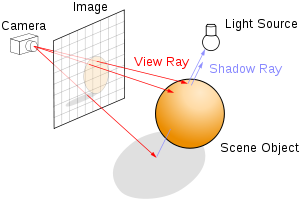
\includegraphics[width=6cm]{raytracing.png}}}%
    \qquad
    \subfloat{{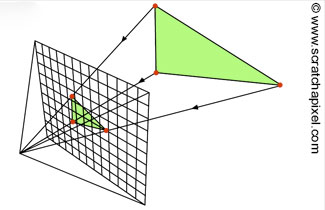
\includegraphics[width=6cm]{rasterization.png}}}%
    \caption{Raytracing (left) vs. Rasterization (right)}%
    \label{fig:example}%
\end{figure}

\begin{figure}[!htbp]
 \centering
 \subfloat{{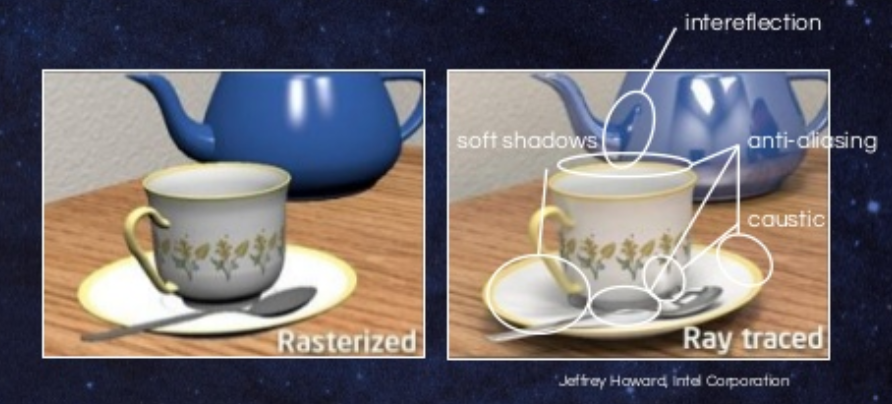
\includegraphics[width=7.5cm,height=3cm]{compare.png}}}
\end{figure}

\section{Raytracing}

\subsection{Algorithm Structure}
\begin{algorithm}[H]
    \SetKwFunction{ray}{createRay}
    \SetKwFunction{inside}{intersect}

    \ForEach{pixel in image} {
        $ray$ \leftarrow \ray{camera, pixel}\\
        \BlankLine
        \ForEach{object in scene} {
            \If{\iside{ray, object} }{
                $image[pixel] \leftarrow object.color$\\
            }
        }
    }
    \caption{Raytracing algorithm}\label{algo_raster}
\end{algorithm}

\subsection{Rendering Spheres}
Spheres are the simplest to raytrace. To formualate if a ray intersects a sphere, lets first define the equation of the sphere as $|\vec{x} - \vec{c}|^2 = r^2$ where $\vec{c}$ is the center and $r$ the radius. The ray can be expressed as $\vec{x} = \vec{s} + t\vec{d}$ where $\vec{s}$ is the camera location,  $\vec{d}$ the unit vector that points from the camera to the pixel, and t the distance from the camera to the point of intersection. Thus,

$$ |\vec{s}+t\vec{d}-\vec{c}| = r^2$$

If we let $\vec{v} = \vec{s} - \vec{c}$, then (unbolded terms denote magnitude)

$$v^2 + t^2d^2 + 2t\vec{v}\cdot\vec{d} = r^2$$
$$t^2 + 2(\vec{v}\cdot\vec{d})t + (v^2-r^2) = 0$$

We can solve for $t$ using the quadratic formula. If $t$ is positive, then we have an intersection, otherwise the sphere is behind the camera. We can then use $t$ to solve for $x$, which can be used for additional considerations (e.g. reflections).

\begin{figure}[!htbp]
 \centering
 \subfloat{{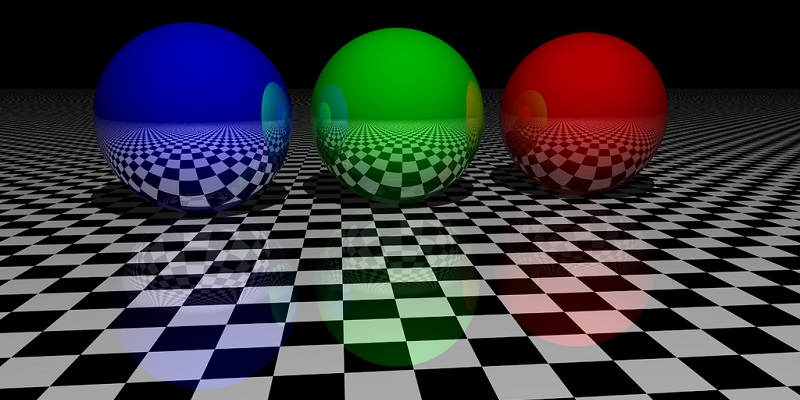
\includegraphics[width=6cm]{spheres.png}}}
 \caption{Raytracing Spheres with reflection and floor texture.}%
 \label{fig:example}%
\end{figure}

\subsection{Barycentric Coordinates}
Baycentric Coordinates are central to many algorithms in computer graphics and can be used to express any located on a triangle with 3 scalars. We will be using barycentric coordinates in the Moller-Trumbone ray-triangle intersection algorithm (Section 3.3). We can express a point P with barycentric coordinates using the following equation: $P = wA + uB + vC$, where A, B, and C are the standard coordinates of the vertices of the triangle and $(w, u, v)$ are the barycentric coordinates of the point $P$. The barycentric coordinates $\left(w,u,v\right)$ satisfy the property that $u + v + w = 1$. Note that we can simply express w as $w = 1 - u - v$ to use two variables instead of three. As a result, our barycentric expression of P becomes:
\begin{equation}
    P = \left(1-u-v\right)A + uB + vC
    \label{barycentric}
\end{equation}

\textit{A note on ranges}: The point $P$ is within the triangle if all coordinates $u, v, w$ lie in the range $\left( 0, 1\right]$. If any coordinate is $0$, then $P$ lies on one of the lines that join the vertices. Additionally, if any barycentric coordinate is less than 0 or greater than 1, the point is outside of the triangle.   

\subsection{Rendering Triangles with Moller-Trumbore}
The Moller-Trumbore algorithm (MT) is a fast ray-triangle intersection algorithm which was introduced in 1997 and is still used in benchmarks to compare performances of other methods. The MT algorithm expresses the intersection point, which we will call P, in terms of its barycenctric coordinates using equation \eqref{barycentric}.

If we expand \eqref{barycentric}, we get
\begin{eqnarray*}
P &=& \left(1-u-v\right)A + uB + vC \\
&=& A - uA -vA + uB + vC \\
&=& A+u(B-A)+v(C-A)
\end{eqnarray*}
 We can think of the expression (B-A) as the vector pointing from A to B and (C-A) as the vector pointing from A to C. It makes sense that we can reach any point on the triangle ABC using the coordinates of A and these two vectors. \\
Additionally, the intersection point P may be written using the ray's parametric equation:
\begin{equation*}
    P = O + tD
\end{equation*}
where O is the ray's origin point and t is the distance from the origin point to P. If we equate the ray parameterization of P to the barycentric expansion of P, we come to the following relationship:
\begin{equation*}
    O - A = -tD + u(B-A) + v(C-A)
\end{equation*}
We can solve for the barycentric coordinates and ray parameter (t, u, v) using Cramer's rule by first expressing the relationship with matrices:

$$
\begin{bmatrix}
D & (B-A) & (C-A)
\end{bmatrix}
\begin{bmatrix}
t \\
u \\
v 
\end{bmatrix}
=
\left[ O-A \right]
$$
Solving for $\begin{bmatrix} t &u &v  \end{bmatrix} ^T$ allows us to reconstruct P using equation \eqref{barycentric}.

\subsection{The Polygon Mesh}
Usually, triangles are the polygon of choice for rendering complex scenes because complex objects can be decomposed into triangles using polygon triangulation. For instance, an apple can be made of hundreds or thousands of triangles. This structure is known as a polygon mesh. Multiple polygon meshes may be present in a scene. They are usually stored in an .OBJ file, which gives the vertices of the triangles, faces, and other information for rendering the scene.

\subsection{Shadows and Lighting}
Shadows result naturally from raytracing. If we place light sources in the scene, every time we hit an object, we can determine if the point is illuminated. To do so, we cast a ray from the intersection point to each light source. If each ray does not intersect any object, then the point is illuminated, otherwise shadow.

If the point is illuminated, we can calculate the lighting as a function the light sources (recall from the camera model lecture, this function is known as the Bidirectional Reflectance Distribution Function (BDRF). One of the most famous BDRFs is the Phong Model. Lighting is composed of the diffuse and specular components.
$$ BDRF(x) = K_d*D + K_s*S$$

\newpage

\begin{figure}[!htbp]
 \centering
 \subfloat{{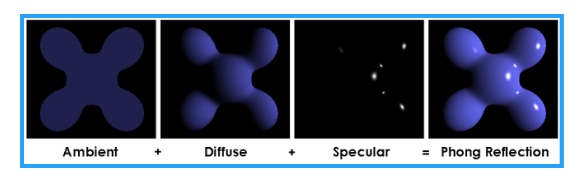
\includegraphics[width=9cm]{phong.png}}}
\end{figure}

\section{Rasterization}

\begin{wrapfigure}{r}{0.325\textwidth}
  \vspace{-25pt}
  \begin{center}
    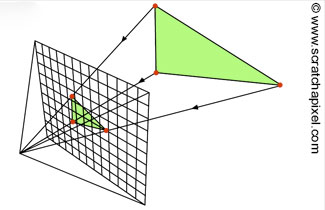
\includegraphics[width=0.3\textwidth]{rasterization.png}
  \end{center}
  \caption{Rasterization}
  \label{rasterization}
  \vspace{-00pt}
\end{wrapfigure}

Rasterization is an alternative method to solve the \textbf{visibility problem}.
While raytracing is image-centric, rasterization is \textbf{object-centric}—fundamentally, this means that instead of starting from the image pixels and trying to determine what objects they contain, we start from the objects in the scene and project them onto the pixels.

Although not quite as photo-realistic as ray tracing, rasterization is still a widely used algorithm due to its performance advantages.
Believe it or not, GPUs weren't originally designed to train ML networks or mine bitcoin, but rather to perform rasterization (the G in GPU stands for Graphics, after all).
As such, the structure and pipeline of GPUs are closely tied to the procedure of rasterization.

\subsection{Algorithm structure}

The rasterization algorithm consists of two main steps:
\begin{enumerate}
    \item \textbf{Projection}—real-world object coordinates are projected onto the image plane.
    This uses the same \textbf{perspective transform} that we've previously encountered on several occasions. 
    \item \textbf{Rasterization}—objects are drawn on the canvas on a pixel-by-pixel basis.
    The term comes from the notion of \textif{raster images}, the common file format that stores images by pixel values (as opposed to vector images).
\end{enumerate}

\begin{algorithm}[H]
    \SetKwFunction{project}{perspectiveProject}
    \SetKwFunction{inside}{insideTriangle}
    
    \tcp{1. Projection}
    \For{triangle3D in scene}{
        $triangle2D$ \leftarrow \project{camera, triangle2D}\\
        \BlankLine
        \tcp{2. Rasterization}
        \ForEach{pixel in image}{
            \If{\inside{triangle2D, pixel} }{
                $image[pixel] \leftarrow triangle2D.color$\\
            }
        }
    }
    \caption{Rasterization algorithm}\label{algo_raster}
\end{algorithm}

Notice the algorithmic effect of being object-centric—our outer loop now iterates over triangles, not pixels.

You may have also noticed that this algorithm is written to only work with triangles.
As it turns out, relying on this simple shape makes computations much easier and faster, while nearly any surface can be adequately represented with small enough triangles.
Specifically, it's very simple to check whether a point lies inside a triangle (that's the \textit{insideTriangle} method from before).
Here are more details if you're interested in the math behind it:
\begin{itemize}
    \item The basis of this procedure is the \textbf{edge function}: a function that determines whether a given point lines to the left or right of a given line (the sides are determined by the order of the two points that define the line).
    \item After sorting the triangle vertices in clockwise order, we know that a point is inside the triangle iff the edge function is \textbf{positive for all 3 triangle sides}.
    \item Recall that $u\times v = \|u\|\|v\|\sin{\theta}$, where $\theta$ is the angle between the two vectors.
    This angle is positive if $u$ is to the right of $v$ and negative if to the left.
    If $v$ the vector between the two line points and $u$ is the one between the first line point and the queried point, the sign of $\theta$ becomes identical to the edge function.
    For $(-\pi, \pi)$, the sign of $sin{\theta}$ is identical to that of $\theta$, so all we have to do for the edge function is find the sign of the \textbf{cross product}.
    \item The cross product has the property of being \textbf{linear}. You don't need to exactly know what this is, but for now, it means that the cross product can easily be parallelized on a GPU. In other words, multiple pixels can be tested at once.
\end{itemize}

\subsection{Bounding Boxes Optimization}

\begin{wrapfigure}{r}{0.35\textwidth}
  \vspace{-45pt}
  \begin{center}
    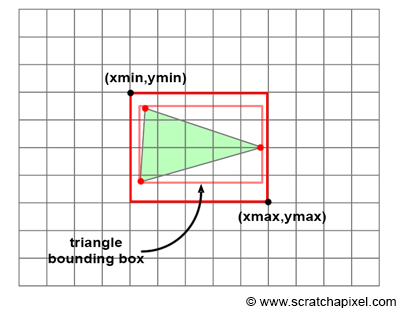
\includegraphics[width=0.35\textwidth]{raster_bounding.png}
  \end{center}
  \vspace{-15pt}
  \caption{Bounding boxes}
  \label{cylinder}
  \vspace{-25pt}
\end{wrapfigure}

In this implementation, we write out our data onto the array \textit{image}.
This is known as an \textbf{image buffer}—it contains the same pixel values that will be displayed at the algorithm's completion.
This array is rather large and we fully iterate over it once for every triangle, this creates a problem when the scene contains many triangles.
for small triangles this is especially wasteful: we end up checking a lot of empty space outside the triangle.

The solution to this is a \textbf{bounding box}: iterate over the smallest rectangular region that contains the triangle.
Its limits correspond to the minimum and maximum x- and y- values of the triangle's vertices.
In practice, don't forget to also cap these at the image limits.

\subsection{Z-buffer}

If there are multiple overlapping triangles in the scene, the order that we draw them in matters.
As such, we need to somehow figure out which triangles are covered by which.

Raytracing solves this visibility problem by drawing the first object each ray encounters, i.e. the object with the \textit{closest distance} along the ray.
Rasterization likewise utilizes real-world distance, but here things become more complicated.
The thing is, we can't solve the problem by simply sorting the drawing order by distance—this breaks when triangles intersect in the 3D space, and as such the overlapping order varies.

What we use instead is a \textbf{distance buffer}, also known as a \textbf{z-buffer}.
Just like the image buffer, it is an array that stores numbers that correspond to each image pixel, only now they represent the real-world distance of each currently drawn pixel.
Now, we also have to check whether new pixels are in front of currently drawn ones before overwriting them.
If they are, we also update the z-buffer.

\begin{algorithm}[H]
    \SetKwFunction{inside}{insideTriangle}
    \SetKwFunction{min}{min}
    \SetKwFunction{max}{max}
    
    \tcp{2. Rasterization}
    $xmin$ \leftarrow \max{$\lfloor$\min{triangle2D.xs}$\rfloor$, 0}\\
    $ymin$ \leftarrow \max{$\lfloor$\min{triangle2D.ys}$\rfloor$, 0}\\
    $xmax$ \leftarrow \min{$\lceil$\max{triangle2D.xs}$\rceil$, image.width}\\
    $ymax$ \leftarrow \min{$\lceil$\max{triangle2D.ys}$\rceil$,
    image.height}\\
    \BlankLine
    \For{xmin \leq x \leq xmax}{
        \For{ymin \leq y \leq ymax}{
            $inside, z$ \leftarrow \inside{triangle2D, (x, y)}\\
            \If{inside}{
                \If{z $< zbuffer[y][x]$}{
                    $zbuffer[y][x] \leftarrow z$\\
                    $image[y][x] \leftarrow triangle2D.color$\\
                }
            }
        }
    }
    \caption{Bounding box and Z-buffer modifications}\label{algo_bounding}
\end{algorithm}

\subsection{Linear Interpolation}

Note that in the previous section, we assumed that \textit{insideTriangle} can somehow extract the needed distance.
How can it do that, if it does not have access to the 3D triangle? 

In practice, computing distances on the 3D triangles is difficult, so we employ \textbf{barycentric coordinates} as a shortcut.

Let's draw 3 lines from the vertices to the queried point, dividing it into 3 smaller triangles.
It just so happens, that the barycentric coefficients exactly correspond to the percentage of the opposing side's triangle's area.
In other words, if we assign three different colors to the vertices, and then mix them according to the coefficients, the triangle will have a nice blend of color that's based on distance to the vertices.

In this situation, we can do the same with distances.
All we need to do is calculate the distances of each vertex in the 3D space, and save them with the projected coordinates.
Now, we can easily interpolate for the distance of any point on the triangle plane.

Furthermore, this computation directly uses triangle area to find the barycentric coordinates.
This is important, as triangle area can be easily found with the cross product. Lucky for us, we've already calculated these cross products when checking whether points lie inside the triangle.

\section{Comparison}

So, which one should you use?

Is one clearly better than the other?

The simple answer is that rasterization is faster, while ray-tracing is better-looking.

The full truth is more complicated.

Firstly, it's true that rasterization is much faster than raytracing. This is due to many years of research and perfection of its algorithms and hardware. Here's what that means:
\begin{enumerate}
    \item Rasterization is currently the only of the two that can comfortably run in real-time.
    If you happen to use any simulation, game, or other product that isn't precomputed, its almost always using rasterization.
    \item Rasterization has already been highly optimized.
    While this is good in itself, it also means that there's probably not as much room for improvement.
\end{enumerate}
Still, it's not that you can't create stunning imagery with rasterization. While the object-centric model quickly gets complicated with the bending or curvature of light (specifically, reflection off of curved surfaces, refraction, black holes), there have been many tricks developed over the years to create products that look nearly as good. The high computational cost of upgrading to raytracing becomes more difficult if the result is not that much better-looking.

Secondly, ray tracing isn't magic.
The interactions of light with objects are complicated—not only are intersections expensive to compute, but it's not always clear what should happen to the light when it hits.
Plain raytracing is going to look plain, unless we also program in shadows, reflections, and various other interactions with materials such as fur or leather.
These things aren't always simple: while things like perfect reflections and refractions are easy, practices such as diffusion and soft shadows require splitting the rays, making the problem exponentially more difficult.
These topics are currently active areas of research, focusing both on how to make raytracing look better, but also how to accelerate them on hardware to make them faster or possible in the first place.
This has allowed raytracing to become popular in situations where quality is far more important than speed, such as in animated movies.

In conclusion, rasterization and raytracing are fundamentally different in their approaches. They are both complicated, but complicated in different places. There has been a lot more research done on rasterization, meaning that while it's faster, raytracing is faster at becoming faster. Overall, it seems that raytracing has a lot more potential for looking better in general, but it's unclear when it will fully replace rasterization, if ever.

\end{document}